\documentclass[10pt,a4paper, norsk]{article}
\usepackage[utf8]{inputenc}
\usepackage{amsmath}
\usepackage[norsk, english]{babel}
\usepackage{geometry, lmodern}
\usepackage[T1]{fontenc}
\usepackage{graphicx}
\usepackage{amsfonts}
\usepackage{amssymb}
\usepackage{listings}
\usepackage{url}
\usepackage{color}
\usepackage[colorlinks=true,linkcolor=black,citecolor=black]{hyperref}
\author{Simen Haugerud Granlund}
\title{TMR4162 - Ramme Analyse}

\hypersetup{
pdfauthor = {Simen Haugerud Granlund},
pdftitle = {TMR4162 - Ramme Analyse},
pdfsubject = {},
pdfkeywords = {},
pdfcreator = {} } 

\begin{document}
\maketitle
\lstset{language=C++,basicstyle=\footnotesize} %\begin{titlepage}
\maketitle
\thispagestyle{empty} 	%fjerner sidetall på første side
\newpage %\end{titlepage}

\section*{Forord}
Dette notatet er laget som en ledd av en innlevering i faget TMR4162 - Prosedyreorientert Programering i 2012. Det inneholder teori og informasjon om et program, kalt FEMA, som utfører en enkel styrkeberegning på en rammekonstruksjon. Programmet kan lastes ned via \url{https://github.com/hgranlund/FEMA}.
\begin{flushright}
Simen Haugerud Granlund, Trondheim 2011.
\end{flushright}
\newpage


\tableofcontents
\newpage


\section{Innledning}
\paragraph{}
Jeg valgte å ta oppgaven "ramme analyse". Grunnen til dette er at jeg synes teorien rundt finite element analyses (FEA) er mye mer interessent og passer bedre til mitt studie enn Poisson-likningen. Jeg valgte også å legge til flere elementer i oppgaven. Oppgaven presiserte at vi bare trengte 2 frihetsgrader per bjelke, samt at vi kun trengte å presentere resultater for bøyemomentet. Jeg valgte å bruke 6 frihetsgrader per bjelke, slik at jeg fikk meg både  vertikal og horisontal forskyvninger og rotasjon. De resultatene jeg ville skulle vises var; Moment diagram, skjærkraft diagram, Normalkraft diagram og starttilstanden. Til dette trenger programmet å regne ut Momenter og normale og aksielle krefter til alle bjelker.

\paragraph{}
Det jeg ville legge mest vekt må under oppgaven var god struktur av koden slik at jeg enkelt kan utvide med nye funksjonaliteter. Med en god struktur er det enkelt å sette seg inn i koden og en slipper å strukturere mye på nytt om en vil legge til nye funksjonaliteter. Jeg liker generelt ikke mye kommentarer i koden. Koden skal være leselig og forstålig uten en hel haug av kommentarer. Selvfølgelig er det steder hvor kommentarer er passende, men generelt holder det med god struktur og navngiving.


\section{Teori}

Her har jeg tenkt å kort beskrive de teoriene som er brukt i programmet. Jeg vil kun ta med de prinsippene, likningene og matrisene jeg brukte i koden og ikke beskrive i detalj hvordan jeg kan frem til dem basert på lærebøker. 


\subsection{Elementmetoden}
Teorien bak elementmetoden ble utarbeidet på 1940-tallet, men man så ikke den store nytteverdien av den før datamaskinen kom til verden. Det første programmet som implementerte elementmetoden var NASTRAN skrevet i Fortran i 1965 \cite{wikinastran}.
Elementmetoden er i prinsippet en numerisk metode for å finne approksimasjoner til differensiallikninger. Den er ofte brukt innenfor en rekke felter: strømning, varmeleding, svinginger, elektriske felt og liknende. I denne oppgaven brukte jeg den for å løse styrkebergnegrer på en rammekonstruksjon. 

\paragraph*{}
Elementmetoden går ut på å dele konstruksjonen inn i elementer, jo flere elementer jo mer nøyaktige resultater får man. Alle elementer har en node i hver ende. Selve rammekonstruksjonen blir representer av et nettverk av noder og elementer, hvor kreftene er festet til nodene. Det er i disse nodene verdier, som forskyving, krefter og momenter, blir kalkulert.

\paragraph*{}
For hvert element blir stivheten til elementet kalkulert. Stivheten er basert på e-modulen, arealet og det andre arealmomentet til elementet. Disse stivhetene blir så addert sammen for å finne systemets stivhet. Vi kan deretter bruke sammenhangen mellom stivhet(k), forskyvninger(v) og krefter(S) \eqref{eq:skv} til å kalkulere knutepunktenes forskyvninger.

\begin{equation} \label{eq:skv}
S=k*v
\end{equation}

\subsubsection{Lokal stivhetsmatrise}
For å regne ut den lokale stivheten til et element kan en bruke stivhetsmatrisen \eqref{eq:Lstivhet}. 

\begin{equation} \label{eq:Lstivhet}
k  = \begin{bmatrix} 
\frac{EA}{L} & 0 & 0 & -\frac{EA}{L} & 0 & 0 \\
0 	& \frac{12EI}{L^3} & -\frac{6EI}{L^2} & 0 & -\frac{12EI}{L^3} & -\frac{6EI}{L^2} \\
0 	&	-\frac{6EI}{L^2} 	& 	\frac{4EI}{L} & 0 & \frac{6EI}{L^2} 	& 	\frac{2EI}{L}\\
-\frac{EA}{L} & 0 & 0 & \frac{EA}{L} & 0 & 0 \\
0 	& -\frac{12EI}{L^3} & \frac{6EI}{L^2} & 0 & \frac{12EI}{L^3} & \frac{6EI}{L^2} \\
0 & -\frac{6EI}{L^2} & \frac{2EI}{L} &0& \frac{6EI}{L^2} & \frac{4EI}{L}
\end{bmatrix}
\end{equation}




Denne stivhetsmatrisen vil nå gjelde lokalt for det enkelte elementet. Vi må derfor transformere matrisen slik at den gjelder globalt. Dette kan vi gjøre med en enkel rotasjonsmatrise \eqref{eq:Rot}. 

\begin{equation} \label{eq:Rot}
R  = \begin{bmatrix}
\cos \theta & -\sin \theta &   0&0&0&0\\[3pt]
\sin \theta & \cos \theta  & 0&0&0&0\\[3pt]
0 &0 & 1&0&0&0\\
0&0&0&\cos \theta & -\sin \theta&   0 \\[3pt]
0&0&0&\sin \theta & \cos \theta  & 0\\[3pt]
0&0&0&0 &0 & 1\\
\end{bmatrix} 
\end{equation}

Vi kan enkelt transformere kreftene $S$ og forskyvningene $v$ ved sammenhengene:
\begin{equation} \label{eq:roteq}
S_G=RS_L  \text{ , } v_G=Rv_L 
\end{equation}

Vi kan nå ved hjelp av \ref{eq:skv} og \ref{eq:roteq} finne en sammenheng mellom den globale $_G$ og den lokale $_L$ stivhetsmatrisen.

\begin{equation}
\begin{aligned}\label{eq:klkg}
& S_G=RS_L=Rk_Lv_L=Rk_LR^{-1}v_G=k_Gv_G \\
&k_G=Rk_LR^{-1}\\
\end{aligned}
\end{equation}

\subsubsection{Global stivhetsmatrise}
Om vi studerer den lokale stivhetsmatrisen \ref{eq:Lstivhet} og likning \ref{eq:skv} ser vi at kolonne nummer $i$ beskriver stivheten til frihetsgraden $i$. Dette er også tilfelle for den globale stivhetsmatrisen. Den globale stivhetsmatrisen holder på stivhetene til alle nodene i systemet, mens den lokale stivhetsmatrise inneholder kun stivheten til sine to tilhørende noder. Når de adderes skal de lokale stivhetene adderes inn i de tilhørende stivhetene i den globale stivhetsmatrisen. Normalt brukes en IEG-matrise, som beskriver systemets topografi, til å addere stivhetene. IEG-matrisen er en relasjon mellom elementene og det tilhørende nodeparret.

\paragraph*{}
Vi kan let kalkulere størrelsen på den globale stivhetsmatrisene. Det første en bør merke seg er at alle stivhetsmatriser er symmetriske, noe som kan bevises ved Maxwells resiprositetssats. Dette her også en følge av newtons 3. lov, siden hver enkelt bjelke må være i likevekt. Det andre er at hver kolonne representerer en frihetsgrad. For å finne størrelsen på matrisen må en derfor beregne antall frihetsgrader til systemet.

\subsubsection{Grensebetingelser}
Nå står vi bare igjen med et lineært ligningssystem av typen $kv=S$, hvor forskyvningene $(v)$ er ukjente. Dette likningssystemet vil nå være uløselig, fordi stivhetsmatrisen $k$ er singulær. Denne singulariteten skyldes at vi enda ikke har sakt hvor konstruksjonen er fastbundet. For et system med 3 frihetsgrader per node trenger vi 3 fastlåste frihetsgrader. Disse frihetsgradene kan innføres på to måter. Enten kan raden og kolonnen til frihetsgraden fjernes, ellers kan alle verdiene nulles ut bortsett fra diagonal-verdien som må være en. Når vi har innført disse grensebetingelsene vil systemet være løselig.

\subsubsection{Elementkrefter}
Når vi vil regne ut krefter på de forskjellige elementene kan vi igjen bruke ligning \ref{eq:skv}. Vi må nå huske at vi må transformere matrisene til det koordinatsystemet vi ønsker. 


\subsection{Ligningsløser}
Når man skal modellere mange fysiske og interiørmessigere problemer kan en nesten ikke unngå å løse store linear ligningssystem. Det finnes derfor mange forskjellige metoder å løse disse på og alle har visse fordeler og ulemper.
Det finnes to kategorier av ligningsløsere: dirkete og iterative. De direkte løser settet eksakt, men bruker ofte lenger tid en en iterativ løser. Gauss metoden er et eksempel på en direkteløser. En iterativ løser finner en approksimasjon av løsningen, og kan ha problemer med konvergens i visse tilfeller. 

\subsubsection{Gauss}

Gauss metoden består av to deler. Den ene er eliminasjon, hvor du utfører elementære rad operasjoner til du for en triangulær form. Deretter gjøres en tilbakesubstitusjon for å finne x-verdiene. De finnes i hovedsak 3 forskjellige rad operasjoner:
\begin{enumerate}
\item Multiplisere en rad med et tall som ikke er null.
\item Addere to rader
\item Bytte om to rader
\end{enumerate}

Kjøretiden til gauss kan kalkuleres ut i fra antall iterasjoner som gjøres. Om vi antar det er $n$ likninger som skal løses kan kjøretiden kalkuleres som vist i \eqref{eq:gausstid}.

\begin{equation} \label{eq:gausstid}
E(n) = \sum_{k=1}^{n-1} (n-k) + 2 \sum_{k=1}^{n-1} (n-k)(n-k-1) = O(n^3)
\end{equation}

På samme måte kan vi kalkulere kjøretiden til tilbakesubstitusjonen:
\begin{equation} \label{eq:gaussseideltid}
T(n) = 2\sum_{i=1}^{n} (n-i) + n = O(n^2)
\end{equation}


\subsubsection{Gauss-Seidel}
Gauss-seidel er en iterativ ligningsløser, som fungerer best på spinkle matriser. Den har en iterativ del, beskrevet i likning \ref{eq:gauss-seidel}. I hver iterasjon bruker Gauss-Seidel  den forrige utregnede verdien, som gjør at den ikke kan kjøre parallelt. 
 
 \begin{equation} \label{seideliterater}
   x_j^{m+1} = \frac{1}{a_{jj}}  (b_j - \sum_{k=1}^{j-1} a_{jk} x_k^{m+1} - \sum_{k=j+1}^n a_{jk}x^m)
 \end{equation}

Her kan vi ikke finne kjøretiden på samme måte som ved en direkteløser, siden vi hele tiden kan forbedre resultatet ved å kjøre en iterasjon til. Vi må derfor se på konvergens, parallellitet og hvilken nøyaktighet man skal ha. Det finnes noen enkle konvergeringsregler for Gauss-Seidel, som sier at metoden garantert konvergerer om:
\begin{enumerate}
\item Matrisen (A) er strengt eller uavvendelige diagonalt dominerende.
\item Matrisen (A) er positive bestemt (Positive-definite)
\end{enumerate}



\subsection{OpenGL}
Opengl er et API for å rendre 2d og 3d grafikk. Mange av kallene går rett på GPU'en, slik at vi får økt ytelsen. Strukturen er bygget opp som en tilstandsmaskin, hvor vi hele tiden forandrer tilstanden til programmet. Vi kan for eksempel sette hvilken farge eller linjetykkelse som skal brukes videre, ved kommandoene glColor3f() og glLineWith().

\paragraph{}
OpenGL opererer med en stakk av 3 matriser, hvor do på hver matrise kan utføre rotasjoner, forskyvninger og skaleringer. Hver gang en matrise operasjon blir kalt blir den utført på den gjeldene matrisen. De forskjellige operasjonene er standard matrise operasjoner, hvor matrisen blir multiplisert med en operasjons matrise.

\begin{equation}
glRotate(\theta	,x,y,z)  = \begin{bmatrix}
1 & 0&  0 &0 \\
0   &\cos \theta &  -\sin \theta &0\\
0 &  \sin \theta   & \cos \theta &0\\
0&0&0&1
\end{bmatrix} * \begin{bmatrix}
\cos \theta  & 0 &  \sin \theta &0\\
0  & 1  & 0 & 0\\
-\sin \theta &  0 &  \cos \theta  &0\\
0&0&0&1
\end{bmatrix} 
*
\begin{bmatrix}
\cos \theta & -\sin \theta &   0 &0\\[3pt]
\sin \theta & \cos \theta  & 0 &0\\[3pt]
0 &0 & 1 &0\\
0&0&0&1\\
\end{bmatrix}
\end{equation}
\begin{equation}
glScale(x,y,z)=
\begin{bmatrix}
x &0&0&0\\
0&y&0&0\\
0&0&x&0\\
0&0&0&1
\end{bmatrix}
\end{equation}
\begin{equation}
glTranslate(x,y,z)=
\begin{bmatrix}
1 &0&0&x\\
0&1&0&y\\
0&0&1&z\\
0&0&0&1
\end{bmatrix}
\end{equation}

For å lage og dytte ut matriser på stakken brukes glPushMatrix() og glPopMatrix(). Når du har hentet ut en matrise kan du utføre rutiner på denne. Modellmatrisen er den mest essensielle matrisen, her kan du utføre rutiner som å tegne streker, polygoner og lignende. 




\section{Programmet} 


\subsection{Beskrivelse}
Dette programmet utfører en enkel styrkeberegning på en en rammekonstruksjon ved hjelp av elementmetoden. Her blir hver bjelke omgjort til et element med 6 frihetsgrader. Analysen kan ta imot krefter eller momenter påsatt i nodene


Programmet er bygget opp av to deler. Det første er en beregnende del, mens den andre er en visualiserende del. Beregningsdelen er skrevet i  Fortran 90 som ut i fra en inputfil utfører en elementanalyse. Resultatene av elementanalysen blir så sendt videre til den visualiserende delen. Denne delen er skrevet i c og viser frem resultatene. 
\subsubsection{Bruk}
\subsubsection{Installasjon}
\subsubsection{Input filen}
Input filen beskriver systemet som skal beregnes. Her skal det spesifiseres hvilke noder, elementer og laster som skal være med i kalkulasjonen. Hvilken benevning som brukes er valgfritt så lenge den er konsekvent. Input filen blir lest igjennom standard input enheten. Figur \ref{fig:input} viser et eksempel på en input fil.

\begin{figure}[h]\label{fig:input}
\centering
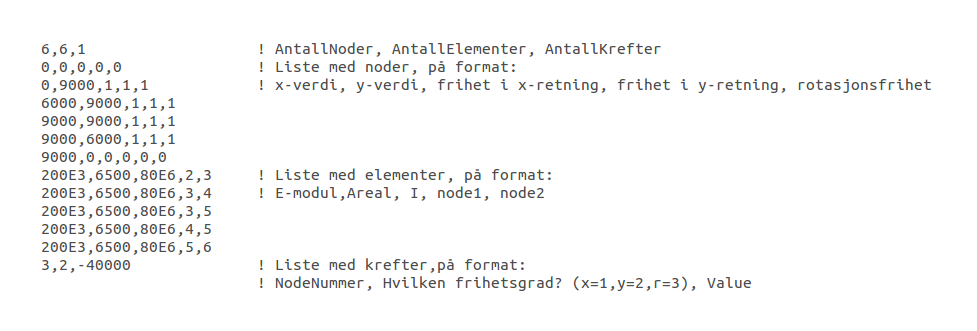
\includegraphics[scale=0.5]{input.png} 
\caption{Eksempel på en input fil}
\end{figure}


\subsection{Fortran}
Delen som er skrevet i fortran implementerer en enkel styrkeberegning basert på elementmetoden. Her er det blant annet også implementert en Ligningsløser som baserer seg på gauss eliminasjon. Her har jeg hentet mye om oppbygging og strukturering fra Kolbein Bell sine notater \cite{KolbeinBellFortran} \cite{KolbeinBellProgram}.  


\subsubsection{Struktur}
Jeg har valgt å strukturere programmet inn i 5 moduler og et hovedprogram. Modulene og hovedprogrammet er delt inn følgende:

\begin{description}
\item[FEM] er navnet på hovedprogrammet mitt. Det er dette programmet som leser og skriver data til fil og kaller på metoder i modulen FEMMetods.
\item[FEMMethods] er hovedmodulen. Dette er den eneste modulen hovedprogrammet bruker. Her finnes alle metoder som har med "finite element method" å gjøre. Hovedrutinen, som utfører styrkeberegningen, heter DoFEA.
\item[FEMUtitity] er en hjelpemodul for FEMMethods. Her finnes alle rutiner som brukes av FEMMethods, men som ikke er koblet direkte opp med FEM. Her er rutiner som for eksempel nullstiler eller printer en matrise.
\item[FEMTypes] er en modul som inneholder de forskjellige datatypene som brukes. De datatypene som brukes er element, joint og load.
\item[FEMMath] er mattemodulen. Her finnes alle rutiner innenfor matematikk som for eksempel rutiner for å utføre gauss eliminasjon eller generere en rotasjonsmatrise.
\end{description}

\paragraph*{}
Jeg har strukturert modulene og programmet som vist i figur \ref{fig:struktur}. Her ser vi at det er hovedprogrammet som tar for seg lesing og skriving til fil og kaller rutinen DoFEA i modulen FEMMethods. DoFEA gjør da de nødvendige kallene for å kalkulere krefter, momenter og forskyvninger på alle elementene. I figuren har jeg ikke tatt med kallene til rutiner som er ubetydelige for forståelsen en strukturen, som for eksempel rutinene i FEMUtility. 

\begin{figure}[h]\label{fig:struktur}
\centering
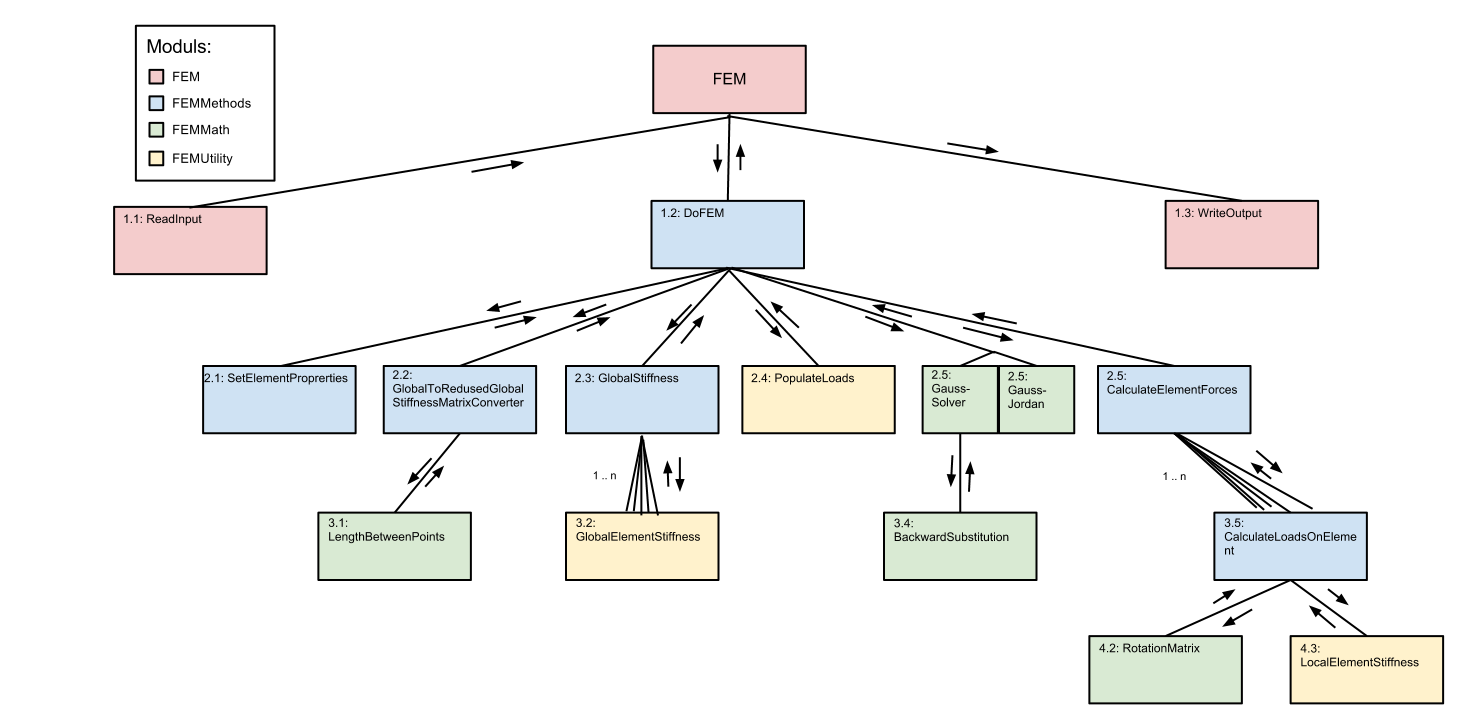
\includegraphics[scale=0.31]{FEMAStructure.png} 
\caption{Program strukturen}
\end{figure}

\paragraph*{}
Datastrukturen jeg har brukt for å representere rammekonstruksjonen og elementene er ved hjelp av egendefinerte datatyper. Den infoen som må holdes på er data om noder, elementer og krefter. Dette har jeg valgt å strukturere ved hjelp av tre datatyper:

\begin{description}
\item[Node] inneholder info om plasseringen til noden, x og y koordinater, og hvilke frihetsgrader noden har.
\item[Element] består av info som tilhører de enkelte elementene som blant annet E-modul, areal , rotasjon og hvilke noder den er koblet til.
\item[Kraft] inneholder hvilken node og retning kraften har og størrelsen på kraften.
\end{description} 

Disse datatypene blir så lagret i tre lister, som blir modifisert og brukt igjennom hele program flyten. Selve programflyten er vist i figure \ref{fig:flytF}. 

\begin{figure}[h]\label{fig:flytF}
\centering
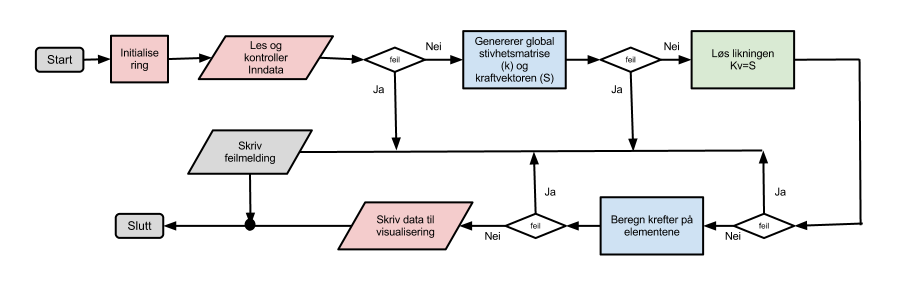
\includegraphics[scale=0.5]{FEMModels.png} 
\caption{Program flyten}
\end{figure}

Her vises også feilhåndterings flyten i programmet. Dette er implementert som anvist i Kolbein \cite{KolbeinBellProgram}, med et errorflagg. 

\begin{align}
& errorflag = 0 : ingen feilsituasjon er påvist \nonumber\\
& errorflag < 0 : en feilsituasjon er påvist\nonumber\\
& errorflag > 0 : en tvilsom situasjon er påvist\nonumber 
\end{align}

\paragraph*{}
Et annet element jeg fant veldig nyttig fra Kolbein \cite{KolbeinBellProgram} var ideen bak variabelen $pr_switch$. Ideen er har at print svitsjen har en verdi mellom 0 og 10, hvor 10 printer alt og 0 ikke printer ut noe. Dette fant jeg veldig nyttig når jeg skulle feilsøke koden. Tanken er at print svitsjene aldri skal bli fjernet slit at det skal bli lett å feil søke koden ved en senere anledning.  



\subsubsection{Program-analyse}

\subsubsection{Optimaliseringer og tidsbruk}
Når vi skal se på den asymptotiske kjøretiden til programmet, er det 2 algoritmer vi må tenke på. Den ene er ligningsløseren, mens den andre er generering av den globale stivhetsmatrisen. Om vi angir $n$ til å være grader av frihet i kunstaksjonen og $e$ til å være antall elementer, kan vi kalkulere kjøretiden. Kjøretiden til Gauss eliminasjonen er vist i \eqref{eq:gausstid}. For stivhetsmatrisen blir alle elementene iterert over og For hvert element addert inn i hovedmatrisen. Kjøretiden blir derfor:

\begin{equation} \label{eq:kjøretidGs}
T(n) = \sum_{k=1}^{e} (k)*(12+12+12+24+24) \sum_{k=1}^{n} (n-k)(n-k) = O(e*n^2)
\end{equation}  

De delene av programmet som har høyest asymptotisk kjøretid er generering av global stivhetsmatrise og ligningsløseren. Jeg har sett litt på hvordan disse kan optimaliseres. 
Den første enkle justeringen jeg gjorde var å kalkulere den globale elementstivhetsmatrisen direkte. Vanligvis ville denne matrisen blitt laget ved å bruke likning \ref{eq:Lstivhet} og \ref{eq:Rot} på formen $k_G=R*k_L*R^T$. Det vil si at vi trenger å gjøre to matrisemultiplikasjoner og en transponering, for å få rotert matrisen. Jeg valgte da å kalkulere denne, på forhånd, slik at $k_G$ blir. 

\begin{equation} 
\begin{aligned}
& k_{with rotation} = \frac{E}{L} * \\ 
&\begin{bmatrix}
AC^2+\frac{12I}{L^2} S^2  & (A-\frac{12I}{L^2})CS  &  -\frac{6I}{L}S & -(AC^2+\frac{12I}{L^2}S^2) & -(A-\frac{12I}{L^2})CS &  -\frac{6I}{L}S \\
 & AS^2 + \frac{12I}{L^2}C^2 & -\frac{6I}{L}S & -(A-\frac{12I}{L^2})CS & -(AS^2+\frac{12I}{L^2}C^2) &  -\frac{6I}{L}S \\
 & & fI &  \frac{6I}{L}S & \frac{6I}{L}C & 2I \\
 & & & (AC^2+\frac{12I}{L^2}S^2) & (A-\frac{12I}{L^2})CS & \frac{6I}{L}S\\
 & & & & (AC^2+\frac{12I}{L^2}C^2) & -\frac{6I}{L}C \\
 Symmetri & & & & & 4I \\
\end{bmatrix} \\
& \mathtt{ Where: E=E-modul, I=Annet arealmoment, } C=cos(\theta), S=\sin(\theta) \\
\end{aligned}
\end{equation}

Dette vil ikke forbedre kjøretiden asymptotisk sett, men vil fjerne noen konstantledd.

\paragraph*{}
En annen ting jeg gjorde var å forbedre genereringen av den globale stivhetsmatrisen. Dette blir vanligvis gjort ved å først lage den fulle matrisen deretter, ved hjelp av grensebetingelser, redusere matrisen. For å unngå to operasjoner lagde jeg den reduserte matrisen direkte. Dette gjorde jeg ved å lage en konverteringsvektor, som mappet verdier fra den tenkte fulle til den reduserte globale stivhetsmatrisen. Jeg laget også en konverteringsvektor fra de de enkelte elementstivhetsmatrisene til den globale stivhetsmatrisen. Dette gjorde at jeg ikke trengte å iterere igjennom hele den globale stivhetsmatrisen hver gang jeg en elementmatrise skulle adderes. 


\paragraph*{}
Det område jeg muligens kunne spare mest tid var å velge en god iterativ ligningsløser. Jeg lagde derfor en implementasjon av gauss-seidel. Teoretisk sett tror jeg det ville vært lurest å gå for en iterativ ligningsløser som Gauss-Seidel. Grunnen til dette er at stivhetsmatrisen som oftest vil være spinkel, siden de fleste frihetsgradene ikke er avhengig av hverandre. De enkelte nodene er kun avhengig av de nærliggende nodene som gjør at vi vil få mage null-verdier i matrisen. Vi vil også få en sterk og alltid utfylt diagonal. Dette er to elementer som er svært positivt for konvergeringen til Gauss-Seidel. Det vil allikevel lønne seg å bruke Gauss eliminasjon på små matriser. Programmet vil derfor, avhengig av størrelsen på stivhetsmatrisen, velge hvilken ligningsløser som er best. 

\paragraph*{}
En annen ting som er vært å peke på når det gjelder fortran, er hvordan matriser traverseres. Fortran bygger matriser i en lang minneblokk med kolonnene etterhandene. Det vil derfor være lurt å traversere kolonne for kolonne. 





\subsubsection{Resultater}



\subsection{C}

\subsubsection{Struktur}
\subsubsection{Optimaliseringer}
\subsubsection{Tidsbruk}

gauss og genereiognav global
\subsubsection{Visualisering}




\subsection{Fargefunksjon}
En fargefunksjon er en funksjon genererer en farge basert på en verdi. Den kan for eksempel returene en rgb verdi. Fargemodellen rgb baserer seg på og blande, blå, grønn og rød, til ønsket farge. 


\section{Diskusjon}

hvorfor jeg valte ting: gauss, innpt stdin

\section{Konklusjon}

lærte nytt tankemønster ved å programere funksjonelt

\paragraph{} 


\begin{thebibliography}{9}

\bibitem{wikinastran}
  Wikipedia,
  \url{http://en.wikipedia.org/wiki/Finite_element_method}
  

\bibitem{waloen}
  Åge Ø. Waløen,
  1995, 
  Dimensjonering ved hjelp av elementmetoden, NTNU
 
\bibitem{FEM}
	Dyryl L. Logen, 2011, A First Course in the Finite Element Method
	
\bibitem{kreyzig}
Erwin Kreyszig, 2006, Advanced Engineering Mathematics, 9th Edition

\bibitem{KolbeinBellProgram}
Kolbein Bell, 2007, Programutvikling (Teknisk, prosedyreorientert programmering), NTNU

\bibitem{KolbeinBellFortran}
Kolbein Bell, 2006, Fortran 90, NTNU

\end{thebibliography}

\end{document}

Dele opp stivhetsmatrise og rotasjonsmatrise i 4 deler


  Det er en del måter å implementere gauss på. Jeg valgte å bruke partiell pivotering, hvor en eliminerer rad for rad men et såkalt pivot element. Dette elementet bør være så stort som mulig for å minske avrundingsfeil. 
  
  
  navngiving
  * Globalelementstivhetsmarise
